% Created 2024-03-14 Thu 18:18
% Intended LaTeX compiler: pdflatex
\documentclass[11pt]{article}
\usepackage{amsmath}
\usepackage[utf8]{inputenc}
\usepackage[T1]{fontenc}
\usepackage{graphicx}
\usepackage{longtable}
\usepackage{wrapfig}
\usepackage{rotating}
\usepackage[normalem]{ulem}
\usepackage{amsmath}
\usepackage{amssymb}
\usepackage{capt-of}
\usepackage{hyperref}
\usepackage{listings}
\usepackage[margin=2.5cm,headheight=66pt]{geometry}
\usepackage{enumitem}
\usepackage{fancyvrb}
\usepackage[magyar, american]{babel}
\usepackage[utf8]{inputenc}
\usepackage[TS1,T1]{fontenc}
\hypersetup{hidelinks=true}
\date{}
\title{Parallel self-adjusting packet classification: Initial results}
\hypersetup{
 pdfauthor={retvari},
 pdftitle={Parallel self-adjusting packet classification: Initial results},
 pdfkeywords={},
 pdfsubject={},
 pdfcreator={Emacs 29.1 (Org mode 9.6.16)}, 
 pdflang={English}}

% Setup for code blocks [1/2]

\usepackage{fvextra}

\fvset{%
  commandchars=\\\{\},
  highlightcolor=white!95!black!80!blue,
  breaklines=true,
  breaksymbol=\color{white!60!black}\tiny\ensuremath{\hookrightarrow}}

% Make line numbers smaller and grey.
\renewcommand\theFancyVerbLine{\footnotesize\color{black!40!white}\arabic{FancyVerbLine}}

\usepackage{xcolor}

% In case engrave-faces-latex-gen-preamble has not been run.
\providecolor{EfD}{HTML}{f7f7f7}
\providecolor{EFD}{HTML}{28292e}

% Define a Code environment to prettily wrap the fontified code.
\usepackage[breakable,xparse]{tcolorbox}
\DeclareTColorBox[]{Code}{o}%
{colback=EfD!98!EFD, colframe=EfD!95!EFD,
  fontupper=\footnotesize\setlength{\fboxsep}{0pt},
  colupper=EFD,
  IfNoValueTF={#1}%
  {boxsep=2pt, arc=2.5pt, outer arc=2.5pt,
    boxrule=0.5pt, left=2pt}%
  {boxsep=2.5pt, arc=0pt, outer arc=0pt,
    boxrule=0pt, leftrule=1.5pt, left=0.5pt},
  right=2pt, top=1pt, bottom=0.5pt,
  breakable}

% Support listings with captions
\usepackage{float}
\floatstyle{plain}
\newfloat{listing}{htbp}{lst}
\newcommand{\listingsname}{Listing}
\floatname{listing}{\listingsname}
\newcommand{\listoflistingsname}{List of Listings}
\providecommand{\listoflistings}{\listof{listing}{\listoflistingsname}}


% Setup for code blocks [2/2]: syntax highlighting colors

\newcommand\efstrut{\vrule height 2.1ex depth 0.8ex width 0pt}
\definecolor{EFD}{HTML}{000000}
\definecolor{EfD}{HTML}{ffffff}
\newcommand{\EFD}[1]{\textcolor{EFD}{#1}} % default
\definecolor{EFh}{HTML}{7f7f7f}
\newcommand{\EFh}[1]{\textcolor{EFh}{#1}} % shadow
\definecolor{EFsc}{HTML}{228b22}
\newcommand{\EFsc}[1]{\textcolor{EFsc}{\textbf{#1}}} % success
\definecolor{EFw}{HTML}{ff8e00}
\newcommand{\EFw}[1]{\textcolor{EFw}{\textbf{#1}}} % warning
\definecolor{EFe}{HTML}{ff0000}
\newcommand{\EFe}[1]{\textcolor{EFe}{\textbf{#1}}} % error
\definecolor{EFc}{HTML}{b22222}
\newcommand{\EFc}[1]{\textcolor{EFc}{#1}} % font-lock-comment-face
\definecolor{EFcd}{HTML}{b22222}
\newcommand{\EFcd}[1]{\textcolor{EFcd}{#1}} % font-lock-comment-delimiter-face
\definecolor{EFs}{HTML}{8b2252}
\newcommand{\EFs}[1]{\textcolor{EFs}{#1}} % font-lock-string-face
\definecolor{EFd}{HTML}{8b2252}
\newcommand{\EFd}[1]{\textcolor{EFd}{#1}} % font-lock-doc-face
\definecolor{EFm}{HTML}{008b8b}
\newcommand{\EFm}[1]{\textcolor{EFm}{#1}} % font-lock-doc-markup-face
\definecolor{EFk}{HTML}{9370db}
\newcommand{\EFk}[1]{\textcolor{EFk}{#1}} % font-lock-keyword-face
\definecolor{EFb}{HTML}{483d8b}
\newcommand{\EFb}[1]{\textcolor{EFb}{#1}} % font-lock-builtin-face
\definecolor{EFf}{HTML}{0000ff}
\newcommand{\EFf}[1]{\textcolor{EFf}{#1}} % font-lock-function-name-face
\definecolor{EFv}{HTML}{a0522d}
\newcommand{\EFv}[1]{\textcolor{EFv}{#1}} % font-lock-variable-name-face
\definecolor{EFt}{HTML}{228b22}
\newcommand{\EFt}[1]{\textcolor{EFt}{#1}} % font-lock-type-face
\definecolor{EFo}{HTML}{008b8b}
\newcommand{\EFo}[1]{\textcolor{EFo}{#1}} % font-lock-constant-face
\definecolor{EFwr}{HTML}{ff0000}
\newcommand{\EFwr}[1]{\textcolor{EFwr}{\textbf{#1}}} % font-lock-warning-face
\newcommand{\EFnc}[1]{#1} % font-lock-negation-char-face
\definecolor{EFpp}{HTML}{483d8b}
\newcommand{\EFpp}[1]{\textcolor{EFpp}{#1}} % font-lock-preprocessor-face
\newcommand{\EFrc}[1]{\textbf{#1}} % font-lock-regexp-grouping-construct
\newcommand{\EFrb}[1]{\textbf{#1}} % font-lock-regexp-grouping-backslash
\newcommand{\EFob}[1]{#1} % org-block
\definecolor{EFhn}{HTML}{008b8b}
\newcommand{\EFhn}[1]{\textcolor{EFhn}{#1}} % highlight-numbers-number
\definecolor{EFhq}{HTML}{9370db}
\newcommand{\EFhq}[1]{\textcolor{EFhq}{#1}} % highlight-quoted-quote
\definecolor{EFhs}{HTML}{008b8b}
\newcommand{\EFhs}[1]{\textcolor{EFhs}{#1}} % highlight-quoted-symbol
\definecolor{EFrda}{HTML}{707183}
\newcommand{\EFrda}[1]{\textcolor{EFrda}{#1}} % rainbow-delimiters-depth-1-face
\definecolor{EFrdb}{HTML}{7388d6}
\newcommand{\EFrdb}[1]{\textcolor{EFrdb}{#1}} % rainbow-delimiters-depth-2-face
\definecolor{EFrdc}{HTML}{909183}
\newcommand{\EFrdc}[1]{\textcolor{EFrdc}{#1}} % rainbow-delimiters-depth-3-face
\definecolor{EFrdd}{HTML}{709870}
\newcommand{\EFrdd}[1]{\textcolor{EFrdd}{#1}} % rainbow-delimiters-depth-4-face
\definecolor{EFrde}{HTML}{907373}
\newcommand{\EFrde}[1]{\textcolor{EFrde}{#1}} % rainbow-delimiters-depth-5-face
\definecolor{EFrdf}{HTML}{6276ba}
\newcommand{\EFrdf}[1]{\textcolor{EFrdf}{#1}} % rainbow-delimiters-depth-6-face
\definecolor{EFrdg}{HTML}{858580}
\newcommand{\EFrdg}[1]{\textcolor{EFrdg}{#1}} % rainbow-delimiters-depth-7-face
\definecolor{EFrdh}{HTML}{80a880}
\newcommand{\EFrdh}[1]{\textcolor{EFrdh}{#1}} % rainbow-delimiters-depth-8-face
\definecolor{EFrdi}{HTML}{887070}
\newcommand{\EFrdi}[1]{\textcolor{EFrdi}{#1}} % rainbow-delimiters-depth-9-face
\begin{document}

\maketitle
\setitemize{noitemsep,topsep=0pt,parsep=0pt,partopsep=0pt}
\selectlanguage{magyar}
\frenchspacing

\section*{Setup}
\label{sec:org8b54939}
\begin{itemize}
\item UDP traffic:
\begin{itemize}
\item 108 bytes
\item dst port varies
\end{itemize}
\item traffic gen: T-REX, 4mpps to overload SUT
\item NIC hashes on UDP dst ports: \texttt{ethtool -{}-{}config-nfc enp7s0 rx-flow-hash udp4 n}
\end{itemize}

\section*{Fitting the modified Amdahl's law}
\label{sec:orgbdb51af}

\begin{itemize}
\item we seek the scaling law in the following general form:
$$S(k) = \frac{\lambda}{s + \frac{1-s}{k^\alpha}}$$
where \(\lambda\) is the performance with a single CPU/thread, \(s\) defines the "sequential" portion of
the code, and \(\alpha\) is the parameter indicating whether the scaling law is indeed superlinear
as follows:
\begin{itemize}
\item \(\alpha=1\): "traditional" Amdahl's law
\item \(\alpha=2\): ideal case (achievable in practice in a "pure" MTF scenario)
\item \(1 < \alpha < 2\): "superlinear scaling"
\end{itemize}
\item we minimize the mean-square-error to fit measured data to the generalized law
\end{itemize}

\section*{Results}
\label{sec:org671e70b}

\subsection*{997 rules, 997 flows, max 8 cpus, DEBUG off}
\label{sec:org6ae85d7}
\begin{itemize}
\item fitted parameters: \(s=0.00424\), \(\alpha=1.458\), \(\lambda=55.16\) [Mbps]
\end{itemize}

\begin{center}
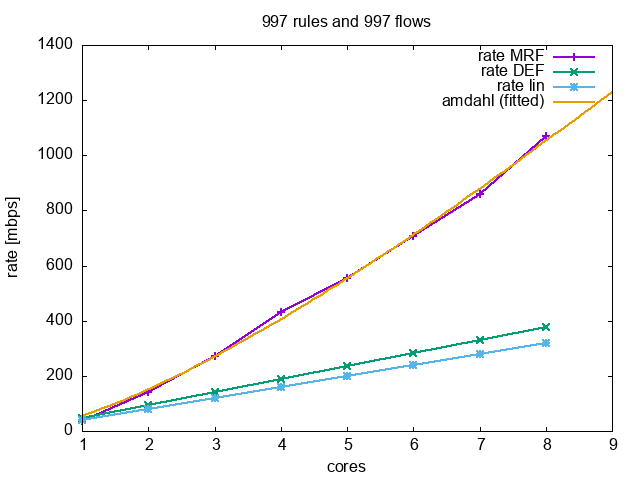
\includegraphics[width=.9\linewidth]{plot-997rules-997flows.png}
\end{center}

\begin{Code}
\begin{Verbatim}
\color{EFD}\EFk{import} numpy \EFk{as} np
\EFk{import} matplotlib.pyplot \EFk{as} plt
\EFk{from} scipy.optimize \EFk{import} curve\_fit
\EFk{import} pandas \EFk{as} pd

\EFk{def} \EFf{SuperLinearAmdahl}(x, *params):
  \EFk{return} params[2] / (params[0] + (1-params[0])/\EFb{pow}(x, params[1]))

\EFv{D} = pd.DataFrame(data)
\EFv{parameters}, \EFv{covariance} = curve\_fit(SuperLinearAmdahl, D[0].to\_numpy(), D[1].to\_numpy(), [0.5,1,1])
\EFb{print}(parameters)
\EFb{print}(covariance)
\end{Verbatim}
\end{Code}

\subsection*{1999 rules, 1999 flows, max 23 cpus, DEBUG off}
\label{sec:org54c7199}
\begin{itemize}
\item fitted parameters: \(s=0.0061\), \(\alpha=2\), \(\lambda=30.9\) [Mbps]
\end{itemize}
\begin{center}
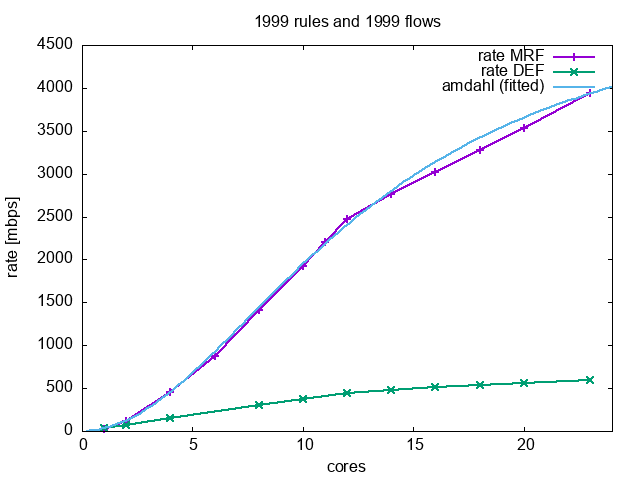
\includegraphics[width=.9\linewidth]{plot-1999rules-1999flows-2.png}
\end{center}

\begin{Code}
\begin{Verbatim}
\color{EFD}\EFk{import} numpy \EFk{as} np
\EFk{import} matplotlib.pyplot \EFk{as} plt
\EFk{from} scipy.optimize \EFk{import} curve\_fit
\EFk{import} pandas \EFk{as} pd

\EFk{def} \EFf{SuperLinearAmdahl}(x, *params):
  \EFk{return} params[2] / (params[0] + (1-params[0])/\EFb{pow}(x, params[1]))

\EFv{D} = pd.DataFrame(data)
\EFv{parameters}, \EFv{covariance} = curve\_fit(SuperLinearAmdahl, D[0].to\_numpy(), D[1].to\_numpy(), [0.5,1,1])
\EFb{print}(parameters)
\EFb{print}(covariance)
\end{Verbatim}
\end{Code}

\subsection*{997 rules, 997 flows, max 23 cpus, DEBUG off}
\label{sec:org13f056f}
\begin{itemize}
\item fitted parameters: \(s=0.0088\), \(\alpha=1.85\), \(\lambda=66.08\) [Mbps]
\end{itemize}
\begin{center}
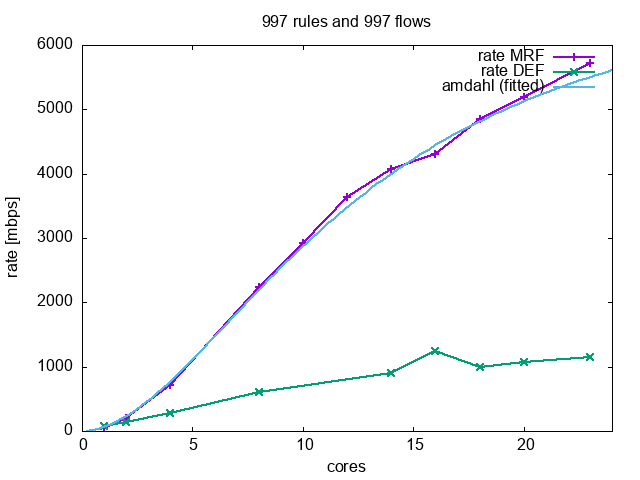
\includegraphics[width=.9\linewidth]{plot-997rules-997flows-rhea-2.png}
\end{center}

\begin{Code}
\begin{Verbatim}
\color{EFD}\EFk{import} numpy \EFk{as} np
\EFk{import} matplotlib.pyplot \EFk{as} plt
\EFk{from} scipy.optimize \EFk{import} curve\_fit
\EFk{import} pandas \EFk{as} pd

\EFk{def} \EFf{SuperLinearAmdahl}(x, *params):
  \EFk{return} params[2] / (params[0] + (1-params[0])/\EFb{pow}(x, params[1]))

\EFv{D} = pd.DataFrame(data)
\EFv{parameters}, \EFv{covariance} = curve\_fit(SuperLinearAmdahl, D[0].to\_numpy(), D[1].to\_numpy(), [0.5,1,1])
\EFb{print}(parameters)
\EFb{print}(covariance)
\end{Verbatim}
\end{Code}


\section*{TODOs}
\label{sec:orga29c1fc}
paper todos:
\begin{itemize}
\item setup TIPSY
\begin{itemize}
\item use classbench integration
\end{itemize}
\item load-balancer? (depends on classbench)
\item prepare two kernels:
\begin{itemize}
\item debug: lock tracing, SAL\textsubscript{DEBUG}, etc.
\item performance: current kernel
\end{itemize}
\item evaluation
\begin{itemize}
\item realistic traffic:
\begin{itemize}
\item classbench flows
\end{itemize}
\item artificial traffic:
\begin{itemize}
\item diff configs:
\begin{itemize}
\item \#nft rules,
\item \#flows,
\item \#controlled flows -> rule duplication
\end{itemize}
\item 1 cpu multiple queues?
\end{itemize}
\end{itemize}
\end{itemize}
\end{document}
